\section{Introduction}

La conception et la mise en œuvre d’une infrastructure moderne reposent aujourd’hui sur l’automatisation complète des processus de création, de configuration et de sécurisation des environnements. Cette approche permet de garantir la cohérence, la traçabilité et la reproductibilité des déploiements tout en réduisant la complexité opérationnelle.

Ce chapitre présente la démarche adoptée pour concevoir et automatiser l’infrastructure du projet, en s’appuyant sur les principes de l’Infrastructure as Code et sur des outils spécialisés. Il expose dans un premier temps les technologies sélectionnées, telles que Proxmox, Terraform, Cloud-init, Ansible, Vault et Consul, qui constituent les fondations techniques de l’architecture. La suite du chapitre décrit la mise en œuvre progressive des différents composants : la gestion des secrets, la création automatisée des machines virtuelles, la préparation des inventaires et la configuration des services.

Par ailleurs, l’usage de Vault comme solution centralisée de gestion des secrets répond à la nécessité de renforcer la sécurité et la traçabilité des informations sensibles au sein de l’infrastructure. Contrairement aux mécanismes de stockage natifs (par exemple les secrets Kubernetes ou les variables d’environnement chiffrées de manière basique), Vault permet de chiffrer systématiquement les données au repos et en transit, de générer des identifiants dynamiques à durée de vie limitée et de contrôler finement les accès via des politiques granulaires. Cette approche réduit les risques de compromission, simplifie la rotation périodique des secrets et garantit que ceux-ci ne transitent jamais en clair dans les dépôts de code ou les configurations partagées. L’intégration de Vault s’inscrit donc pleinement dans la logique Infrastructure as Code et contribue à élever le niveau de sécurité tout en automatisant la distribution des secrets.

Enfin, une attention particulière est portée aux aspects réseau et à la sécurisation des flux, avec l’intégration de pare-feu, de mécanismes d’équilibrage de charge et de politiques de segmentation. Cette démarche globale vise à démontrer qu’il est possible de déployer une infrastructure complète et sécurisée de manière déclarative, tout en facilitant son évolutivité et sa maintenance.
\section{Les outils utilisés pour l’infrastructure as code}

\subsection{Proxmox}

Proxmox Virtual Environment (Proxmox VE) est une plateforme open source de virtualisation et de gestion d’infrastructure qui combine la virtualisation basée sur des machines virtuelles (KVM) et la conteneurisation légère (LXC) dans une interface unifiée. Elle offre une solution complète pour déployer et administrer des environnements virtualisés, qu’ils soient utilisés en laboratoire, en PME ou dans des centres de données. Proxmox se distingue par sa simplicité de mise en œuvre, sa richesse fonctionnelle et sa capacité à fédérer plusieurs nœuds dans un cluster haute disponibilité.

Proxmox répond à plusieurs enjeux stratégiques : rationalisation des ressources matérielles par la mutualisation, réduction des coûts grâce à une solution libre, amélioration de la flexibilité opérationnelle et simplification de la gestion des infrastructures. Son interface web ergonomique permet de piloter l’ensemble des ressources, de planifier les sauvegardes et de superviser les performances.

D’un point de vue technique, Proxmox repose sur plusieurs composantes clés :
\begin{itemize}
	\item \textbf{KVM (Kernel-based Virtual Machine)} : moteur de virtualisation complète.
	\item \textbf{LXC (Linux Containers)} : conteneurisation système légère.
	\item \textbf{Ceph Storage} : stockage distribué intégré et hautement disponible.
	\item \textbf{Cluster Management} : fédération et basculement automatique.
	\item \textbf{Interface Web et API REST} : administration centralisée.
	\item \textbf{Sauvegardes et snapshots} : gestion de la résilience.
\end{itemize}

\textbf{Cas d’utilisation} : déploiement d’un cluster de trois nœuds Proxmox avec stockage Ceph pour héberger des machines virtuelles critiques en haute disponibilité.

\subsection{Terraform}

Terraform est un outil open source d’Infrastructure as Code développé par HashiCorp. Il permet de définir et de provisionner des ressources complètes sous forme de code déclaratif, avec un modèle unifié pour divers fournisseurs (clouds publics, hyperviseurs privés).

Terraform répond à plusieurs enjeux : accélération du provisioning, fiabilisation des configurations et maîtrise des environnements. Il repose sur des concepts clés :
\begin{itemize}
	\item \textbf{Fichiers de configuration (HCL)} : description de l’état souhaité.
	\item \textbf{Providers} : modules d’interface avec les APIs.
	\item \textbf{State file} : enregistrement des ressources créées.
	\item \textbf{Plan d’exécution} et \textbf{apply} : gestion des changements.
	\item \textbf{Modules et workspaces} : factorisation et isolation.
\end{itemize}

\textbf{Cas d’utilisation} : provisionner un cluster Kubernetes sur Proxmox avec un réseau et des volumes configurés.

\subsection{Cloud-init}

Cloud-init est un outil d’initialisation automatique des machines virtuelles lors du premier démarrage. Il est supporté par la plupart des plateformes cloud et hyperviseurs, et permet notamment :
\begin{itemize}
	\item La configuration réseau.
	\item La création d’utilisateurs et de clés SSH.
	\item L’installation de paquets et le lancement de scripts personnalisés.
\end{itemize}

Cloud-init contribue à standardiser les environnements et réduire les délais de mise en service. Il joue également un rôle essentiel comme étape préalable avant l’utilisation d’outils d’infrastructure as code tels que Terraform, en garantissant que les instances disposent d’une configuration de base cohérente (accès SSH opérationnel, configuration réseau correcte, packages requis déjà installés). Cette préparation est indispensable pour que Terraform puisse ensuite se connecter aux machines et appliquer les ressources et configurations supplémentaires de manière automatisée.

\textbf{Cas d’utilisation} : automatiser l’installation de Docker et la configuration réseau d’une instance Proxmox, afin de préparer l’environnement avant l’orchestration et la gestion avancée via Terraform.

\subsection{Ansible}

Ansible est un outil open source d’automatisation et de configuration des systèmes, basé sur un langage déclaratif YAML et une architecture agentless (connexion SSH). Il permet de :
\begin{itemize}
	\item Définir des playbooks réutilisables.
	\item Orchestrer la configuration de plusieurs hôtes.
	\item Gérer des inventaires et des variables.
	\item Assurer la traçabilité des opérations.
\end{itemize}

\textbf{Cas d’utilisation} : configurer des serveurs applicatifs, installer les dépendances et sécuriser les accès.

\subsection{Vault}

Vault est un gestionnaire de secrets développé par HashiCorp, conçu pour sécuriser, stocker et contrôler l’accès aux informations sensibles telles que les identifiants, les clés d’API ou les certificats. Il centralise le cycle de vie des secrets au sein d’un système unique et auditable, tout en offrant des capacités de distribution dynamique et de rotation automatique.

\textbf{Principales fonctionnalités} :
\begin{itemize}
	\item Chiffrement systématique des données au repos et en transit.
	\item Génération dynamique de credentials à durée de vie limitée.
	\item Contrôle d’accès fin grâce à des politiques (ACL) granulaires.
	\item Rotation périodique et automatique des secrets.
	\item Audit complet des opérations et des accès.
\end{itemize}

\subsection{Concepts de base}

Vault repose sur plusieurs concepts fondamentaux :

\begin{itemize}
	\item \textbf{Seal et Unseal} : lors de son démarrage, Vault est scellé (sealed). Dans cet état, aucune donnée ne peut être lue ou écrite. Le processus d’unseal consiste à déverrouiller Vault en fournissant une combinaison de clés de déchiffrement (unseal keys) générées lors de l’initialisation. Ce mécanisme s’appuie sur l’algorithme de \emph{Shamir’s Secret Sharing}, qui divise la clé maîtresse en fragments distribués à différents opérateurs. Cela garantit qu’aucun individu ne détient seul la capacité de déverrouiller le système. La nécessité d’unseal manuellement après un redémarrage contribue à limiter l’exposition en cas de compromission.
	\item \textbf{Backends de stockage} : Vault peut s’appuyer sur différents backends de stockage (par exemple Consul, fichiers locaux, Amazon S3) pour persister ses données chiffrées. Le choix du backend influence les performances, la disponibilité et la tolérance aux pannes.
	\item \textbf{Secrets Engines} : ce sont les composants responsables de la gestion des secrets. Certains engines fournissent du stockage statique (par exemple les clés stockées manuellement), d’autres génèrent des secrets dynamiques à la demande (par exemple des credentials temporaires pour une base de données).
	\item \textbf{Auth Methods} : ces méthodes définissent comment les utilisateurs ou applications s’authentifient auprès de Vault. Il peut s’agir de tokens statiques, d’authentification AppRole, de certificats TLS ou d’intégrations avec Kubernetes.
	\item \textbf{Policies} : les politiques d’accès contrôlent avec précision ce que chaque entité est autorisée à faire. Elles définissent les droits de lecture, d’écriture ou de suppression sur des chemins spécifiques.
\end{itemize}

Vault supporte également un mode haute disponibilité (HA) distribué, qui permet le déploiement d’un cluster avec plusieurs instances. Dans ce mode, un nœud actif (active node) prend en charge les requêtes, tandis que les autres nœuds fonctionnent en standby. Cette architecture contribue à améliorer la tolérance aux pannes, à garantir la continuité de service en cas de défaillance d’un serveur et à renforcer la résilience globale du système.
\subsection{Design de sécurité}

Vault adopte une approche de sécurité par défaut :
\begin{itemize}
	\item Toutes les données sont chiffrées avec une clé maîtresse qui n’est jamais stockée en clair.
	\item Chaque requête est soumise à une évaluation des politiques d’accès.
	\item Les secrets peuvent être versionnés et révoqués à tout moment.
	\item Les logs d’audit permettent de tracer finement chaque opération.
	\item Vault est également capable de générer des \textbf{secrets temporaires} (secrets dynamiques) qui remplacent les identifiants statiques. Ces secrets éphémères expirent automatiquement après un délai défini et peuvent être révoqués de façon proactive, ce qui limite la fenêtre d’exposition en cas de compromission.
\end{itemize}

Ce modèle de sécurité réduit le risque d’exposition accidentelle et renforce la conformité aux exigences réglementaires.

\subsection{Exemple d’utilisation}

Vault est particulièrement adapté pour :
\begin{itemize}
	\item Stocker et distribuer les tokens Kubernetes nécessaires à l’accès au cluster.
	\item Générer des credentials temporaires pour une base de données PostgreSQL.
	\item Chiffrer les certificats TLS utilisés par des applications.
	\item Mettre en place un PKI interne pour l’émission automatique de certificats.
\end{itemize}

\subsection{Bonnes pratiques de sécurité}

Pour garantir un niveau de protection élevé, il est recommandé de :
\begin{itemize}
	\item Distribuer les clés de scellage (unseal keys) à plusieurs opérateurs de confiance afin de prévenir tout point de défaillance individuel.
	\item Configurer une rotation périodique des clés maîtresses.
	\item Limiter strictement l’accès aux méthodes d’authentification les plus sensibles.
	\item Activer et surveiller systématiquement les logs d’audit.
	\item S’assurer que le backend de stockage est hautement disponible et correctement sécurisé.
\end{itemize}

\subsection{Limitations et vigilance}

Si Vault n’est pas configuré de manière rigoureuse, il peut devenir un point unique de défaillance et un vecteur d’attaque majeur. La compromission d’un nœud ou la perte des clés de déchiffrement peut entraîner une indisponibilité prolongée, voire la perte irrémédiable de certains secrets. Il est donc essentiel d’envisager des scénarios de récupération, tels que la sauvegarde chiffrée des données et la documentation des procédures d’unseal.
\subsection{Consul}

Consul est une solution de service discovery, de configuration distribuée et de service mesh développée par HashiCorp. Elle permet de centraliser la gestion dynamique des services et de renforcer la cohérence des environnements déployés. Consul apporte plusieurs fonctionnalités complémentaires à Vault et s’intègre naturellement dans les architectures automatisées.

\subsection{Principales fonctionnalités}

Les principales capacités de Consul sont les suivantes :
\begin{itemize}
	\item \textbf{Découverte automatique des services} : Consul maintient un catalogue des services enregistrés, avec leurs adresses et ports associés, facilitant leur détection et leur utilisation par d’autres composants.
	\item \textbf{Supervision de l’état des services} : le système exécute des contrôles de santé (health checks) qui permettent de vérifier en continu la disponibilité et le bon fonctionnement des instances.
	\item \textbf{Stockage clé-valeur} : Consul fournit un KV store distribué, utilisé pour stocker des paramètres de configuration ou des informations dynamiques accessibles par les applications.
	\item \textbf{Service mesh sécurisé} : grâce à l’intégration avec Envoy, Consul offre un plan de contrôle permettant de chiffrer le trafic inter-services, d’implémenter des politiques d’accès et de réaliser du routage avancé.
\end{itemize}

\subsection{Architecture et composants}

Consul repose sur une architecture distribuée, composée de plusieurs éléments :
\begin{itemize}
	\item \textbf{Agents} : chaque nœud du cluster exécute un agent Consul, qui peut être configuré en mode client ou serveur.
	\item \textbf{Serveurs} : les serveurs Consul assurent la cohérence des données à l’aide d’un consensus basé sur le protocole Raft.
	\item \textbf{Catalogue de services} : une base de données en temps réel contenant les informations sur tous les services enregistrés et leur état de santé.
	\item \textbf{KV Store} : un espace de stockage distribué, utilisé pour partager des données de configuration.
	\item \textbf{Connect} : le composant de service mesh qui gère l’émission de certificats TLS, le chiffrement du trafic et le contrôle des autorisations.
\end{itemize}

\subsection{Mécanismes et cas d’usage}

Consul propose plusieurs mécanismes qui répondent à des besoins spécifiques :

\begin{itemize}
	\item \emph{Service discovery} : lorsqu’un service s’enregistre auprès de Consul, il devient automatiquement visible pour les clients qui peuvent interroger l’API DNS ou HTTP afin de récupérer ses coordonnées.
	\item \emph{Health checks} : chaque enregistrement de service peut être associé à un ou plusieurs tests de disponibilité. Si un service échoue aux contrôles, il est retiré du catalogue actif.
	\item \emph{KV Store} : les applications peuvent récupérer dynamiquement des paramètres ou configurations partagées (par exemple des variables d’environnement ou des endpoints).
	\item \emph{Consul Template} : cet outil surveille le KV store et les catalogues, puis génère automatiquement des fichiers de configuration lorsque des changements surviennent.
	\item \emph{Service mesh} : Consul Connect émet des certificats mTLS, configure les proxys Envoy et applique des politiques d’accès qui définissent quels services sont autorisés à communiquer.
\end{itemize}

\textbf{Exemple d’utilisation} : synchroniser dynamiquement les configurations applicatives avec Consul Template, mettre à jour les fichiers de configuration NGINX lorsque de nouveaux services sont enregistrés, ou établir un canal de communication chiffré entre des microservices.

\subsection{Bonnes pratiques de sécurité}

Pour tirer parti des fonctionnalités de Consul tout en maintenant un niveau élevé de sécurité, il est recommandé de :
\begin{itemize}
	\item Activer le chiffrement TLS pour toutes les communications inter-nœuds.
	\item Protéger l’interface HTTP API par une ACL stricte.
	\item Mettre en place des politiques de token management et de rotation régulière des secrets.
	\item Limiter l’accès aux agents et serveurs Consul au sein d’un réseau privé.
	\item Activer l’audit des requêtes et opérations critiques.
\end{itemize}

\subsection{Limitations et vigilance}

De meme que vault , malgré sa richesse fonctionnelle, Consul peut devenir un point unique de coordination : une indisponibilité du cluster impacte la découverte des services et la cohérence des configurations. De plus, une configuration incorrecte des ACL ou des intentions (politiques de service mesh) peut entraîner des fuites d’informations ou des interruptions de service. Il est donc essentiel de soigner le dimensionnement du cluster, de planifier des sauvegardes régulières et de tester les scénarios de bascule.

\section{Mise en place des concepts de l'infrastructure en code}

La mise en œuvre d'une infrastructure déclarative repose sur une combinaison d'outils spécialisés qui permettent d'automatiser l'ensemble du cycle de vie des environnements techniques. Cette approche favorise la cohérence, la traçabilité et la reproductibilité des déploiements.
Les sections suivantes décrivent les principales étapes mises en place dans le projet.

\subsection{Préparation des secrets avec Vault}

Dans une architecture moderne, la gestion sécurisée des informations sensibles (mots de passe, clés d'API, certificats) est un enjeu majeur.
Pour répondre à cette problématique, l'outil HashiCorp Vault a été utilisé comme coffre-fort centralisé.

Vault a été configuré en mode \textit{server} avec un stockage interne et une politique de chiffrement des données au repos. Les secrets sont créés et organisés dans des chemins logiques (\texttt{secret/}, \texttt{kv/}) permettant de les isoler par projet ou par environnement (développement, production).

L'accès à Vault est contrôlé par des policies granulaires, et l'authentification des outils d'automatisation (Terraform, Ansible) s'effectue via des tokens dynamiques ou l'approche AppRole.
Cette centralisation simplifie la rotation des secrets et réduit les risques liés aux configurations manuelles.

\subsection{Création de templates de machines virtuelles}

Afin de garantir l'uniformité des systèmes de base, des templates de machines virtuelles ont été préparés sur Proxmox.
Ces templates incluent :
\begin{itemize}
	\item Le système d'exploitation minimal (par exemple Debian ou Ubuntu LTS).
	\item Les mises à jour de sécurité appliquées.
	\item Les dépendances de base (cloud-init, agents QEMU, agents SPICE et agents ).
	\item La configuration des clés SSH nécessaires à l'automatisation.
\end{itemize}

L'utilisation de ces modèles préconfigurés permet de créer rapidement de nouvelles instances sans avoir à répéter les étapes de préparation initiale.
Cette approche contribue à standardiser le socle technique et à réduire le temps de provisionnement.

\subsection{Création des machines virtuelles à travers Terraform}

La création automatisée des machines virtuelles est orchestrée par Terraform.
Les ressources sont décrites sous forme de fichiers HCL (\textit{HashiCorp Configuration Language}) qui précisent :
\begin{itemize}
	\item La taille et le nombre de vCPU et de mémoire.
	\item Le réseau et les interfaces associées.
	\item Le disque principal et son format.
	\item Le template de base à cloner.
\end{itemize}

L'exécution de \texttt{terraform apply} permet de matérialiser l'infrastructure déclarée.
Cette étape est également responsable de l'injection initiale des métadonnées (par exemple, le nom de l'instance, l'identifiant d'environnement).
Grâce à Terraform, la création des VMs est reproductible et contrôlée dans le temps.

\subsection{Préparation automatique des inventaires}

Après le provisionnement des ressources, la préparation des inventaires est essentielle pour permettre à Ansible de prendre le relais.
Pour ce faire, un script d'automatisation collecte dynamiquement les informations des machines créées (adresses IP, identifiants, groupes logiques) et génère un inventaire au format YAML compatible avec Ansible.

Cette génération automatisée évite les erreurs liées aux manipulations manuelles et garantit que l'inventaire reflète toujours l'état réel de l'infrastructure.De plus, elle s’inscrit dans une démarche DRY (Don’t Repeat Yourself), en éliminant la duplication des informations entre les étapes de provisionnement et de configuration
L'inventaire est versionné dans un dépôt Git, renforçant la traçabilité des évolutions.

\subsection{Configuration automatique des machines virtuelles avec Ansible}

Une fois les inventaires préparés, Ansible est utilisé pour configurer les machines virtuelles de manière déclarative.
Les rôles et playbooks appliquent notamment :
\begin{itemize}
	\item La création des utilisateurs et des groupes.
	\item La configuration du pare-feu et des règles de sécurité.
	\item L'installation des paquets requis.
	\item Le déploiement des configurations d’applications et des services système.
\end{itemize}

L'exécution d'Ansible est idempotente, garantissant que les machines convergent toujours vers l'état souhaité, quelle que soit leur configuration initiale.
Les variables sensibles sont injectées de manière sécurisée via Vault.

\section{Outils de réseau, exposition des services et sécurité}

Le bon fonctionnement d'une infrastructure passe par une gestion rigoureuse du réseau et une exposition contrôlée des services.
Dans le projet, plusieurs composants et bonnes pratiques ont été mis en œuvre :

\begin{itemize}
	\item \textbf{Réseau virtuel et segmentation} : les machines sont placées dans des VLANs distincts afin de séparer les environnements (production, développement) et de limiter les flux inter-zones.
	\item \textbf{Reverse proxy et ingress} : l’exposition des services HTTP(S) s’effectue via des ingress controllers Kubernetes ou des reverse proxies tels que NGINX. Ces composants assurent le routage, la terminaison TLS et l’équilibrage de charge.
	\item \textbf{Certificats TLS} : les certificats sont gérés automatiquement grâce à l’intégration de Let’s Encrypt ou Vault PKI, garantissant la sécurité des échanges.
	\item \textbf{Pare-feu et contrôle des accès} : des règles strictes sont appliquées sur les hôtes et les pods, combinant iptables, security groups et Network Policies Kubernetes.
	\item \textbf{Monitoring et logs} : la collecte centralisée des logs réseau et la supervision des connexions permettent d’anticiper les incidents et de renforcer la sécurité.
\end{itemize}

Cette approche cohérente assure une exposition minimale des services au public et une sécurité renforcée tout en maintenant une haute disponibilité.

\subsection{Firewall pfSense}

Pour renforcer la sécurité réseau, plusieurs architectures avec \textbf{pfSense} (distribution libre spécialisée dans les fonctions de pare-feu et de routage) ont été considérées. Voici les options analysées :

\subparagraph{Scénario 1 : pfSense en VM ou LXC dédié sur Proxmox}

\begin{itemize}
	\item pfSense est déployé comme une VM avec deux interfaces réseau (WAN et LAN).
	\item Elle agit comme passerelle pour toutes les autres VMs.
	\item Avantage : isolation logique et grande flexibilité.
	\item Limite : dépendance à Proxmox (si le nœud tombe, le firewall aussi).
\end{itemize}

\subparagraph{Scénario 2 : pfSense sur un serveur physique séparé}

\begin{itemize}
	\item pfSense fonctionne comme appliance physique devant le cluster.
	\item Avantage : indépendance vis-à-vis de la plateforme de virtualisation.
	\item Permet de filtrer tout le trafic entrant/sortant.
	\item Limite : nécessite du matériel dédié, plus de câblage et de gestion physique.
\end{itemize}

\begin{figure}[H]
	\centering
	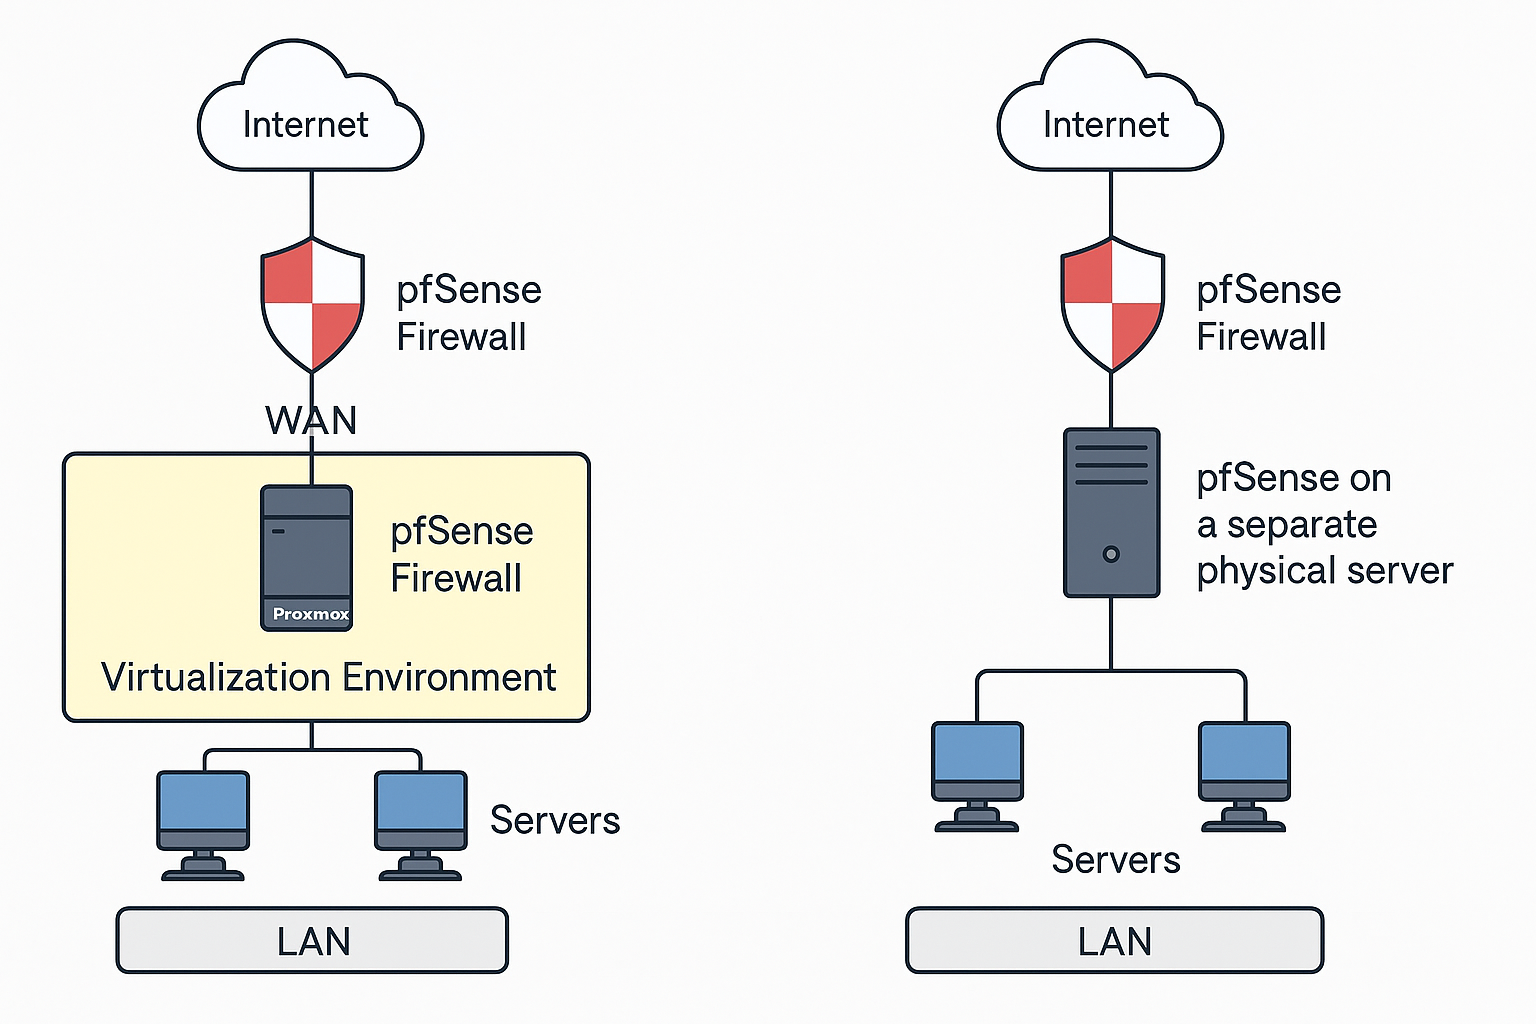
\includegraphics[width=0.85\textwidth]{figures/choix implementation pfsense.png}
	\caption{Comparaison des architectures d'intégration de pfSense}
\end{figure}

Le tableau \ref{tab:pfsense_arch} résume les avantages et inconvénients de chaque approche :

\begin{longtable}{|p{4.5cm}|p{3.5cm}|p{3cm}|p{3.5cm}|}
	\caption{\it{Comparaison des modes d’intégration de pfSense}}
	\label{tab:pfsense_arch}                                                                                                               \\ \hline
	\textbf{Architecture}        & \textbf{Isolation} & \textbf{Résilience} & \textbf{Commentaires}                                        \\ \hline
	\endfirsthead
	\multicolumn{4}{l}{\tablename\ \thetable\ -- \textit{Suite}}                                                                           \\ \hline
	\textbf{Architecture}        & \textbf{Isolation} & \textbf{Résilience} & \textbf{Commentaires}                                        \\ \hline
	\endhead
	\endfoot
	\hline
	\endlastfoot

	VM dédiée ou LXC sur Proxmox & Élevée             & Moyenne             & Facile à déployer, centralisé, mais dépend du nœud Proxmox.  \\ \hline
	Appliance physique séparée   & Très élevée        & Très élevée         & Solution professionnelle, coûteuse, idéale pour multi-sites. \\ \hline
\end{longtable}

\subsection{Choix retenu et justification}

Dans le contexte de l’infrastructure actuelle de Oneex, c’est le \textbf{scénario 1} (déploiement de pfSense dans une VM dédiée sur Proxmox) qui a été retenu. Cette approche présente plusieurs avantages majeurs en adéquation avec l’architecture existante :

\begin{itemize}
	\item Elle permet d’\textbf{intégrer pleinement le pare-feu dans le réseau interne}, avec un contrôle précis sur le filtrage inter-VLAN et la segmentation réseau.
	\item pfSense peut \textbf{établir des connexions VPN de type IPsec} entre les différents LANs internes de l’entreprise, assurant ainsi une interconnexion sécurisée des environnements distants.
	\item Cette configuration est \textbf{hautement personnalisable} : routage, NAT, tunnels chiffrés, DHCP statique, filtrage applicatif, etc., tout en restant cohérente avec la logique IaaS de Proxmox.
\end{itemize}

Malgré une résilience moyenne (liée à sa dépendance à Proxmox), cette solution constitue un compromis optimal entre flexibilité, centralisation et sécurité, tout en réduisant les coûts matériels. Elle est également plus facile à maintenir et à intégrer dans les processus automatisés de l'infrastructure.

\subsection{Réseau de Kubernetes}

Le réseau Kubernetes est un élément fondamental qui permet la communication entre les différents composants du cluster et les applications qui y sont déployées. Il repose sur plusieurs concepts clés visant à simplifier la connectivité et à assurer l’isolation logique des workloads.

\subsection{Modèle de réseau plat}

Kubernetes adopte un modèle de réseau dit \emph{plat}, dans lequel :
\begin{itemize}
	\item Chaque \textbf{pod} reçoit une adresse IP unique.
	\item Tous les pods peuvent communiquer entre eux, sans traduction d’adresses (NAT).
	\item Les pods peuvent accéder aux services exposés par d’autres pods, quel que soit le nœud sur lequel ils s’exécutent.
\end{itemize}
\begin{figure}[H]
	\centering
	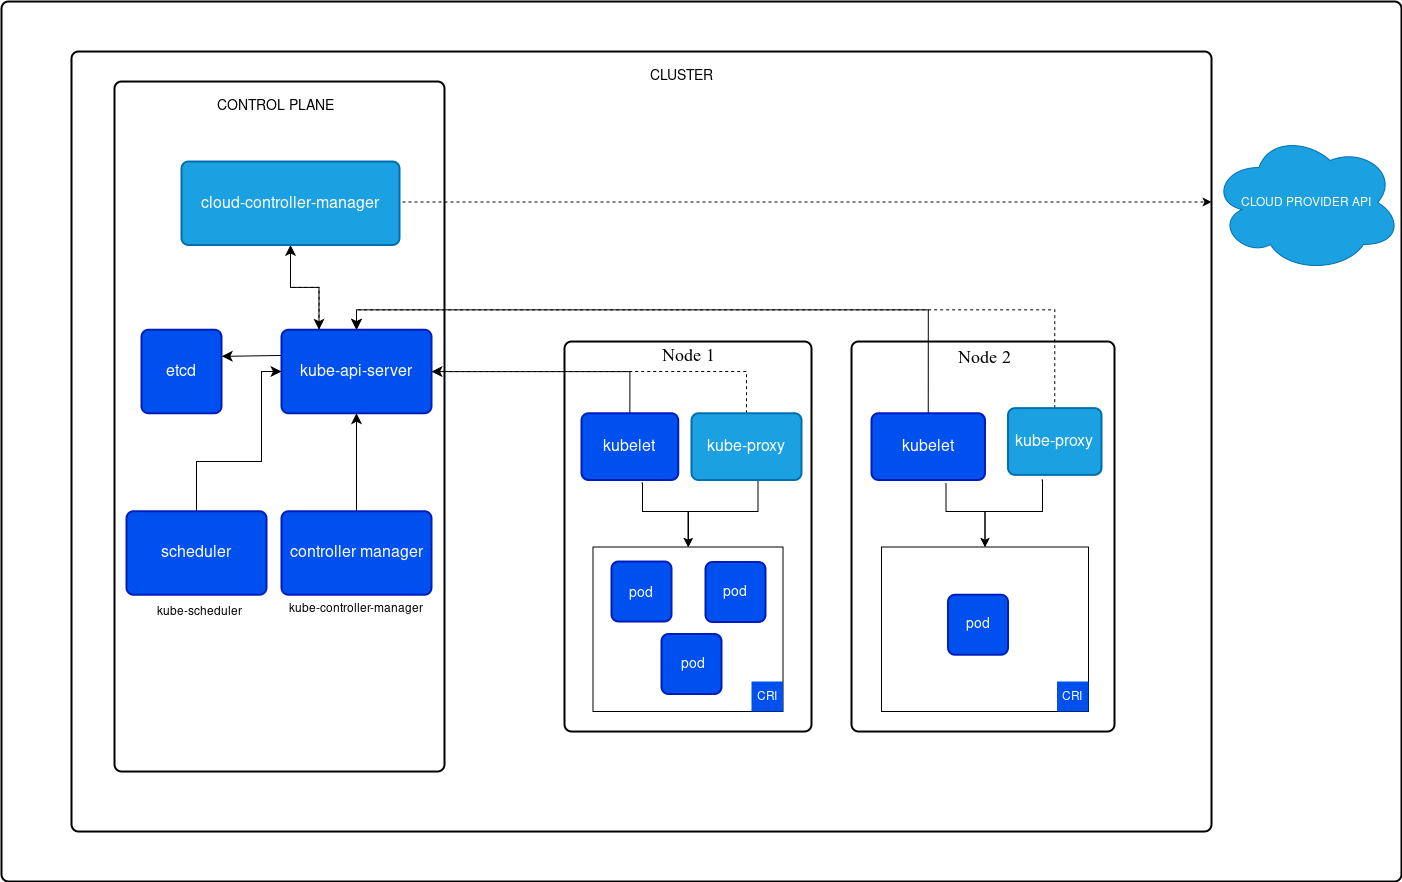
\includegraphics[width=0.85\textwidth]{figures/kubernetes-cluster-architecture.png}
	\caption{Architecture d'un cluster Kubernetes}
\end{figure}
Ce modèle vise à réduire la complexité des communications et à permettre aux applications de se comporter comme si elles fonctionnaient sur un même réseau local.

\subsection{CNI (Container Network Interface)}

Pour mettre en œuvre le modèle réseau, Kubernetes s’appuie sur des plugins CNI (Container Network Interface).
Ces plugins sont responsables de :
\begin{itemize}
	\item L’attribution des adresses IP aux pods.
	\item La configuration des routes réseau.
	\item L’application des règles de filtrage ou d’isolation.
\end{itemize}
Parmi les solutions CNI les plus courantes, on peut citer Calico, Flannel, Cilium et Weave.

\subsection{Services et exposition réseau dans Kubernetes}

Kubernetes introduit l’objet \texttt{Service}, utilisé pour exposer un ensemble de pods via une abstraction réseau stable (nom DNS et IP virtuelle). Cela permet de découpler la logique de service de l’adressage dynamique des pods.

\begin{figure}[H]
	\centering
	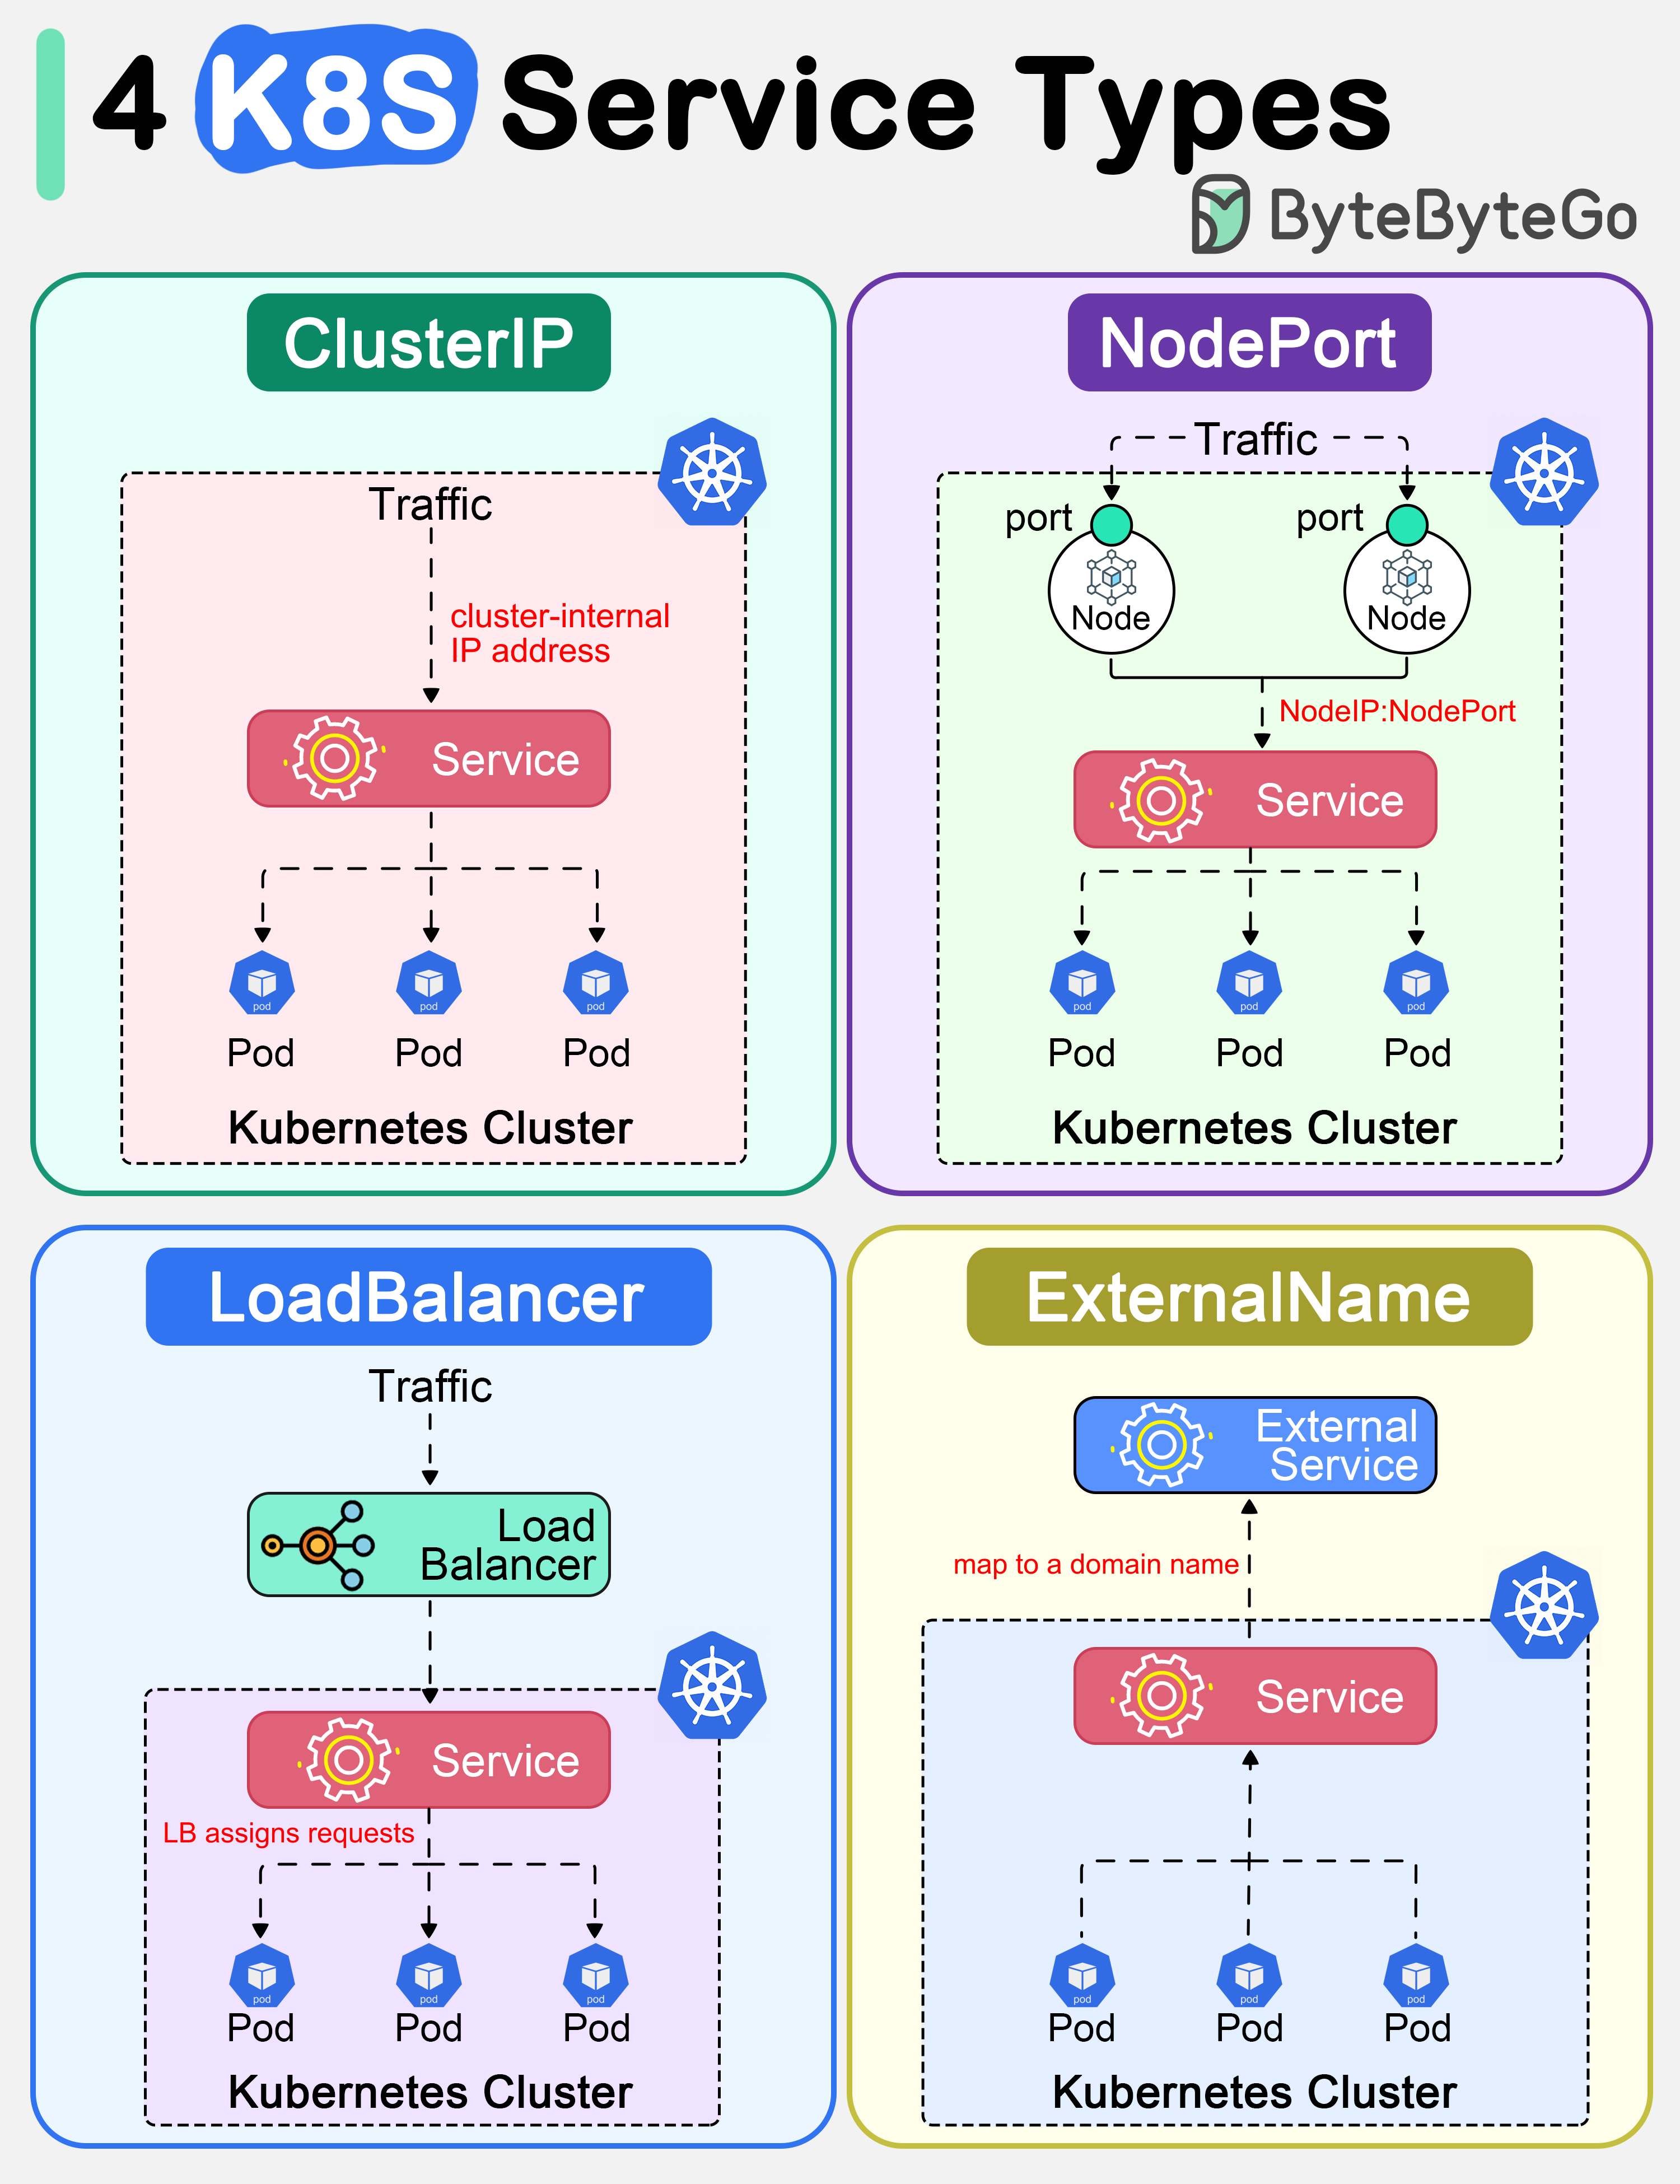
\includegraphics[width=0.85\textwidth]{figures/k8s-service-types.png}
	\caption{Types de services Kubernetes}
\end{figure}

\subparagraph{ClusterIP}
Il s’agit du type de service par défaut. Il crée une IP virtuelle interne au cluster, accessible uniquement depuis les autres composants Kubernetes. Le routage est effectué via le composant \texttt{kube-proxy}, qui configure des règles \texttt{iptables} ou \texttt{IPVS} selon la configuration du cluster.

\subparagraph{NodePort}
Ce type expose le service sur un port statique (généralement entre 30000 et 32767) sur toutes les interfaces réseau de chaque nœud. Le trafic externe accède alors aux pods via l’adresse IP d’un nœud et le port attribué.

\subparagraph{LoadBalancer}
Ce type s’appuie sur l’intégration avec un fournisseur de cloud pour provisionner automatiquement un équilibreur de charge (load balancer) et attribuer une IP publique. Il est idéal pour l’exposer à Internet, mais dépend de l’environnement cloud.

\subparagraph{ExternalName}
Ce type ne crée pas réellement de proxy mais agit comme une redirection DNS. Il permet d’exposer un service interne vers une ressource externe en mappant son nom à un domaine DNS externe, sans gestion de pods ou endpoints.

\subparagraph{Ingress}
En complément des services, l’objet \texttt{Ingress} permet de définir des règles de routage HTTP(S) avancées :
\begin{itemize}
	\item Routage basé sur les hôtes ou les chemins.
	\item Terminaison TLS.
	\item Redirections, en-têtes personnalisés, sécurité.
\end{itemize}
Un contrôleur d’Ingress (comme NGINX ou Traefik) est requis pour appliquer ces règles.

\bigskip

\subparagraph{Tableau récapitulatif des types de services Kubernetes}

\begin{longtable}{|p{4cm}|p{5cm}|p{6cm}|}
	\caption{\it{Comparatif des types de services Kubernetes}}
	\label{tab:services_k8s}                                                                                                                      \\ \hline
	\textbf{Type de service} & \textbf{Accessibilité}                  & \textbf{Utilisation typique}                                             \\ \hline
	\endfirsthead
	\multicolumn{3}{l}{\tablename\ \thetable\ -- \textit{Suite}}                                                                                  \\ \hline
	\textbf{Type de service} & \textbf{Accessibilité}                  & \textbf{Utilisation typique}                                             \\ \hline
	\endhead
	\hline \multicolumn{3}{r}{\textit{Suite de la page précédente}}                                                                               \\ \hline
	\endfoot
	\hline
	\endlastfoot

	\texttt{ClusterIP}       & Interne au cluster uniquement           & Communication entre pods ou services backend internes                    \\ \hline
	\texttt{NodePort}        & Accès via IP du nœud et port externe    & Test local, accès direct sans load balancer                              \\ \hline
	\texttt{LoadBalancer}    & IP publique attribuée automatiquement   & Exposition publique dans un environnement cloud                          \\ \hline
	\texttt{ExternalName}    & Redirection DNS vers un service externe & Connexion à des services externes (API tierces, bases de données gérées) \\ \hline

\end{longtable}
Le tableau \ref{tab:services_k8s} présente une comparaison synthétique des différents types de services proposés par Kubernetes.

\subsection{Network Policies}

Pour renforcer la sécurité, Kubernetes propose les \texttt{NetworkPolicies}, qui définissent des règles de filtrage des flux entre pods :
\begin{itemize}
	\item Sélection des pods sources et destinations.
	\item Protocoles et ports autorisés.
	\item Isolation stricte par namespace ou par label.
\end{itemize}
Les politiques réseau nécessitent un CNI compatible (par exemple Calico).

\subsection{DNS interne}

Kubernetes fournit un service DNS interne (CoreDNS) qui résout les noms des services et pods :
\begin{itemize}
	\item Chaque service est accessible via un nom DNS du type \texttt{myservice.mynamespace.svc.cluster.local}.
	\item Les applications peuvent utiliser la découverte de services sans configuration externe.
\end{itemize}

En combinant ces composants, le réseau Kubernetes offre un modèle cohérent, flexible et extensible qui facilite le déploiement d’applications distribuées tout en garantissant la sécurité et l’évolutivité.

\subsection{MetalLB}

MetalLB est une solution de load balancing spécialement conçue pour les clusters Kubernetes déployés en environnement on-premise. Contrairement aux plateformes cloud qui fournissent des services d’équilibrage de charge natifs, les installations locales de Kubernetes ne disposent pas par défaut d’un mécanisme équivalent pour l’attribution d’adresses IP publiques et la distribution du trafic.

\subsection{Principales fonctionnalités}

MetalLB apporte plusieurs fonctionnalités essentielles :
\begin{itemize}
	\item \textbf{Attribution d’adresses IP virtuelles} : il permet de réserver et d’annoncer des plages d’adresses IP utilisables pour exposer les services en mode \emph{LoadBalancer}.
	\item \textbf{Distribution du trafic réseau} : il redirige les requêtes entrantes vers les pods cibles, en fonction de la configuration et de l’algorithme de balancing choisi.
	\item \textbf{Compatibilité BGP et L2} : MetalLB propose deux modes de fonctionnement :
	      \begin{itemize}
		      \item Le mode \textbf{Layer 2}, qui utilise ARP ou NDP pour annoncer l’adresse IP sur le réseau local.
		      \item Le mode \textbf{BGP}, qui permet d’établir des sessions de routage dynamique avec les routeurs de l’infrastructure.
	      \end{itemize}
\end{itemize}

\subsection{Mécanisme de haute disponibilité (HA)}

MetalLB met en œuvre un mécanisme de haute disponibilité pour garantir la continuité de service même en cas de défaillance d’un nœud.

Dans le mode Layer 2 :
\begin{itemize}
	\item Un seul nœud dans le cluster est désigné comme \emph{speaker} pour une adresse IP donnée.
	\item En cas de panne ou d’indisponibilité du nœud speaker, les autres nœuds organisent une élection pour élire un nouveau speaker, qui prendra le relais et continuera à annoncer l’IP virtuelle sur le réseau.
\end{itemize}

Ce mécanisme permet de garantir que les services exposés restent accessibles même en cas de panne matérielle ou logicielle sur un nœud.

\subsection{Avantages et inconvénients}

\begin{itemize}
	\item \textbf{Avantages} :
	      \begin{itemize}
		      \item Permet l’utilisation de services \texttt{LoadBalancer} en on-premise sans équipement physique supplémentaire.
		      \item Haute disponibilité grâce à la redondance des speakers.
		      \item Facilement intégrable dans un cluster Kubernetes existant.
		      \item Compatible avec les politiques réseau Kubernetes.
	      \end{itemize}

	\item \textbf{Inconvénients / Limites} :
	      \begin{itemize}
		      \item \textbf{Goulot d’étranglement potentiel} : seul le speaker actif reçoit le trafic entrant pour une IP donnée, ce qui peut limiter le débit réseau.
		      \item Ce modèle peut réduire le \emph{throughput} maximal, car le speaker redistribue ensuite le trafic vers les pods cibles situés éventuellement sur d'autres nœuds.
		      \item Le modèle ne permet pas un load balancing L4 actif/actif entre nœuds (sauf en mode BGP multi-routeur).
	      \end{itemize}
\end{itemize}

\subsection{Remarque sur les performances}

Dans la majorité des cas d’usage (web APIs, services métiers), la limite du throughput au niveau du speaker est acceptable. En effet, le facteur limitant n’est pas la capacité réseau brute mais le temps de traitement des requêtes applicatives. Grâce au modèle distribué de Kubernetes, ce traitement est réparti entre les pods, ce qui permet de maintenir de bonnes performances globales même si un seul nœud reçoit initialement le trafic.

\begin{figure}[H]
	\centering
	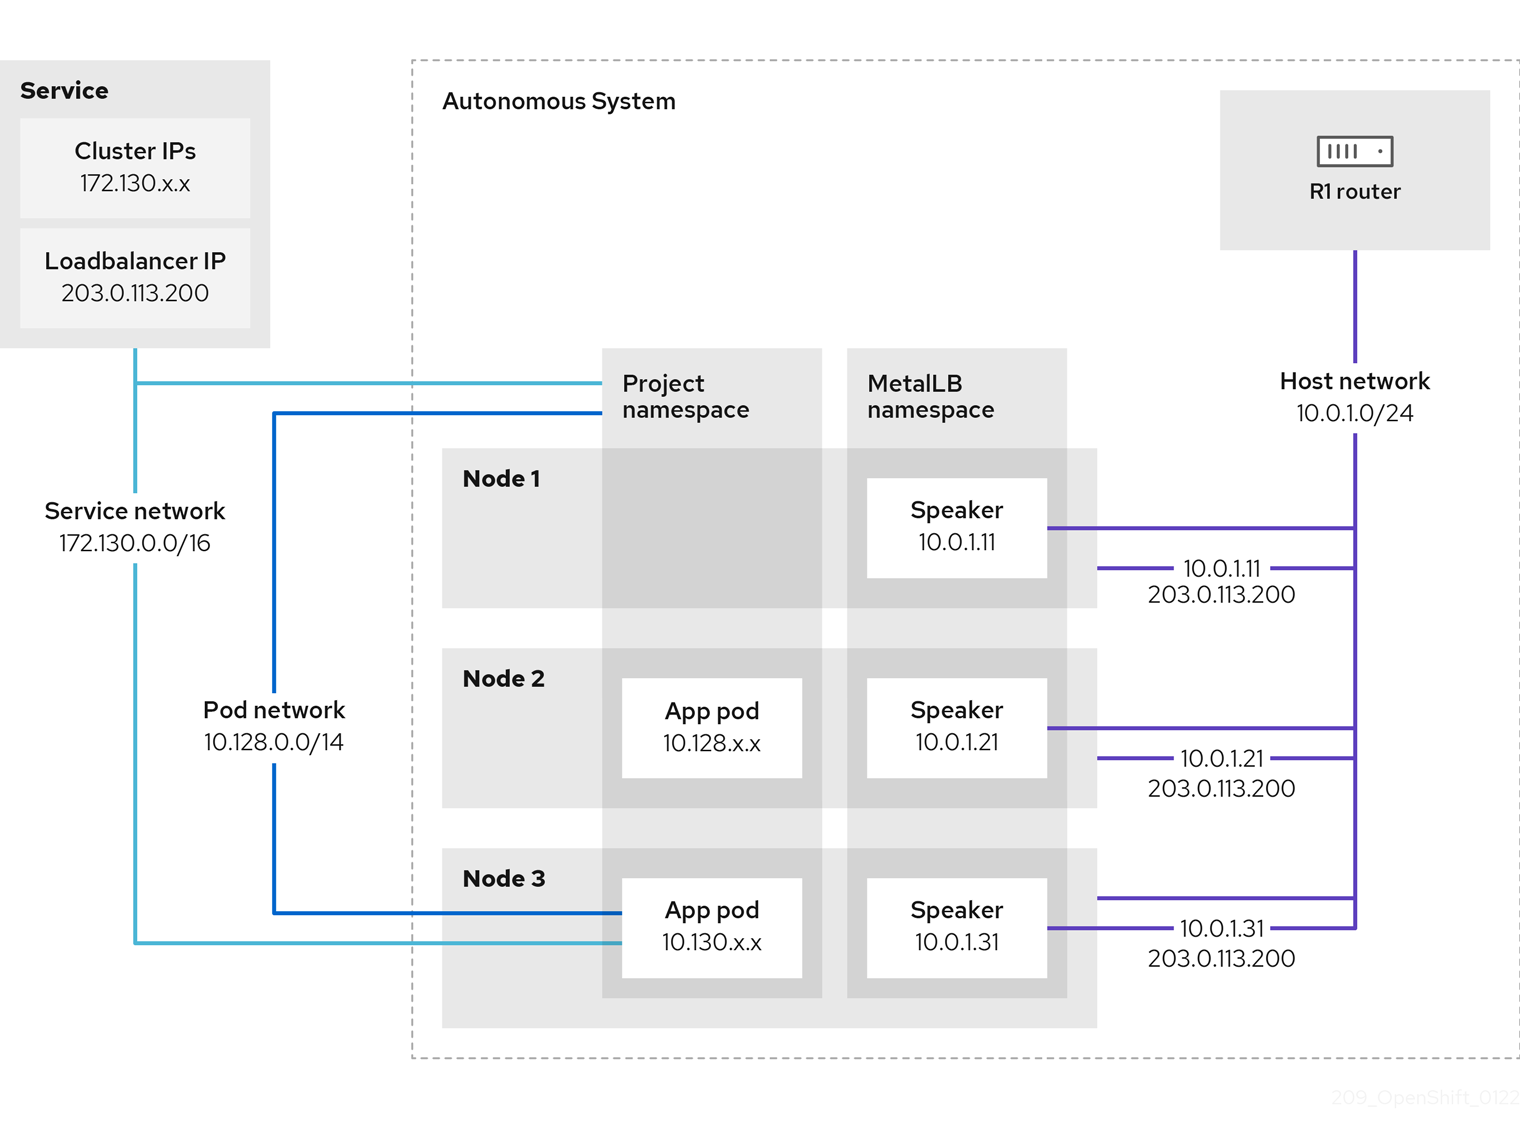
\includegraphics[width=0.85\textwidth]{figures/Metallb network.png}
	\caption{Réseau de MetalLB}
\end{figure}

\section{Mise en place des services de réseau}

Cette partie décrit la mise en œuvre et l’automatisation des services essentiels au bon fonctionnement du réseau et à la sécurisation des flux. Ces services incluent le pare-feu, le reverse proxy ainsi que la gestion centralisée des secrets.

\subsection{Configuration automatique de pfSense avec Ansible}

Le pare-feu pfSense constitue le point d’entrée et de filtrage du trafic réseau. Afin de garantir la reproductibilité de sa configuration et d’éviter les erreurs manuelles, Ansible a été utilisé pour automatiser son déploiement et sa configuration.

Pour cela, des modules spécifiques à pfSense et des collections Ansible dédiées ont été mis en œuvre, permettant notamment :
\begin{itemize}
	\item La définition des règles de filtrage (firewall rules) par groupe et par interface.
	\item La configuration des interfaces réseau et des VLANs.
	\item L’activation et la configuration du service DHCP.
	\item La gestion des utilisateurs et des certificats.
\end{itemize}

Grâce à cette approche, il est possible de versionner les configurations pfSense dans un dépôt Git et de les appliquer de manière cohérente sur plusieurs environnements.
En cas de restauration après sinistre, la remise en service peut ainsi être réalisée rapidement et de façon fiable.

\subsection{Configuration de NGINX avec Ansible}

NGINX joue un rôle central comme reverse proxy et point d’entrée HTTP(S) des applications.
La configuration de NGINX a été automatisée avec Ansible afin de :
\begin{itemize}
	\item Créer et gérer les fichiers de configuration des sites virtuels (server blocks).
	\item Générer automatiquement les certificats TLS via Let’s Encrypt.
	\item Mettre en place les règles de redirection et de réécriture des URLs.
	\item Définir les paramètres de sécurité (headers HTTP, limitation de débit).
\end{itemize}

Les rôles Ansible développés permettent de paramétrer NGINX de manière déclarative en fonction des variables d’inventaire et de secrets provenant de Vault.
Chaque modification de configuration est ainsi versionnée et peut être appliquée de façon idempotente.

\subsection{Usage de Vault pour la gestion des secrets}

La gestion centralisée et sécurisée des secrets est assurée par HashiCorp Vault.
Vault est utilisé comme source unique de vérité pour stocker et distribuer :
\begin{itemize}
	\item Les mots de passe d’accès aux services.
	\item Les clés API nécessaires aux applications.
	\item Les certificats TLS privés.
	\item Les tokens d’authentification.
\end{itemize}

L’authentification des systèmes à Vault s’effectue via AppRole et tokens dynamiques, ce qui limite le risque de compromission en cas de fuite d’identifiants.
Ansible est configuré pour interroger Vault à l’exécution des playbooks et récupérer les secrets de manière transparente.
Cette approche présente plusieurs avantages :
\begin{itemize}
	\item Les secrets ne sont jamais stockés en clair dans les dépôts Git.
	\item La rotation régulière est facilitée.
	\item Les accès sont tracés et audités.
\end{itemize}

L’intégration de Vault avec Terraform et Ansible permet ainsi de garantir un niveau de sécurité élevé tout au long du cycle de vie des environnements.

\section{Synthèse}

La combinaison d’outils tels que Proxmox, Terraform, Ansible, Vault et pfSense a permis de construire une infrastructure automatisée, sécurisée et reproductible. Cette approche s’inscrit dans la démarche Infrastructure as Code, garantissant un haut niveau de cohérence et facilitant les évolutions futures.

\section{Presentation des outils GitOps}
\subsection{Argo CD}

Argo CD est un outil open source de déploiement continu (CD) natif Kubernetes, conçu pour mettre en œuvre les pratiques GitOps. Il permet de synchroniser l’état désiré des applications, défini dans un dépôt Git, avec l’état effectif du cluster Kubernetes. En automatisant la gestion et le déploiement des manifestes, Argo CD apporte cohérence, traçabilité et résilience aux environnements cloud-native.

%point de vue metier
Argo CD répond à plusieurs enjeux stratégiques  : fiabiliser les déploiements, réduire le temps de mise en production, renforcer la traçabilité et limiter les erreurs humaines. Il offre un modèle déclaratif et auditable, conforme aux exigences de sécurité et de conformité des organisations modernes. En industrialisant le GitOps, Argo CD contribue à accélérer l’innovation tout en garantissant la stabilité des systèmes.

%point de vue logique et technique
, Argo CD s’appuie sur plusieurs composants clés  :
\begin{itemize}
	\item \textbf{Le dépôt Git}  : source unique de vérité contenant les manifestes Kubernetes (YAML) ou les définitions Kustomize/Helm.
	\item \textbf{Le contrôleur Argo CD}  : composant qui surveille les différences entre l’état souhaité (Git) et l’état réel du cluster.
	\item \textbf{L’API Server et l’interface Web}  : couche d’administration et de visualisation centralisée des applications et des synchronisations.
	\item \textbf{Les applications}  : objets Kubernetes représentant l’état désiré d’un ensemble de ressources.
	\item \textbf{Les stratégies de synchronisation}  : modes automatique ou manuel permettant de contrôler les mises à jour.
\end{itemize}

Argo CD offre un modèle de sécurité avancé, intégrant la gestion fine des permissions (RBAC), le support du SSO (OAuth2, OIDC), le chiffrement des secrets et des validations automatiques des changements.

\textbf{Exemples et cas d’usage} :
\begin{itemize}
	\item Déployer automatiquement une application Helm versionnée depuis un dépôt Git centralisé.
	\item Gérer des environnements multiples (dev, staging, production) avec des dossiers ou des branches distinctes.
	\item Appliquer des politiques de synchronisation automatique avec validation de signature Git.
	\item Visualiser les différences entre l’état courant et l’état cible et lancer un déploiement manuel.
	\item Auditer l’historique des déploiements et des changements appliqués au cluster.
\end{itemize}

\textbf{Avantages principaux} :
\begin{itemize}
	\item Mise en œuvre native du GitOps et centralisation de la configuration déclarative.
	\item Traçabilité et auditabilité complètes des changements.
	\item Intégration fluide avec Helm, Kustomize, Jsonnet et plain YAML.
	\item Réduction du risque d’erreurs grâce au contrôle automatique des dérives d’état.
	\item Interface Web ergonomique et API REST.
	\item Sécurité renforcée avec RBAC et chiffrement des secrets.
\end{itemize}

En synthèse, Argo CD est une solution stratégique pour l’automatisation et la fiabilisation des déploiements Kubernetes. Il contribue à instaurer des workflows GitOps robustes, cohérents et évolutifs, adaptés aux exigences opérationnelles des entreprises modernes.

\textbf{Références suggérées} :
\begin{itemize}
	\item Argo CD Documentation – \url{https://argo-cd.readthedocs.io/}
	\item Argo CD GitHub Repository – \url{https://github.com/argoproj/argo-cd}
	\item GitOps Principles – \url{https://www.gitops.tech/}
	\item CNCF Argo Project – \url{https://www.cncf.io/projects/argo/}
	\item Helm Documentation – \url{https://helm.sh/docs/}
\end{itemize}

\subsection{Helm}

Helm est un gestionnaire de packages Kubernetes qui permet de décrire des applications sous forme de charts. Chaque chart contient des modèles de manifestes et des fichiers de valeurs qui définissent les paramètres de l’application. Helm est particulièrement adapté lorsque :
\begin{itemize}
	\item Les applications déployées nécessitent de nombreuses options configurables.
	\item Il est souhaité de réutiliser des packages officiels ou communautaires (par exemple nginx, prometheus).
	\item Les équipes ont besoin de versionner et de publier des applications sous forme de packages standardisés.
\end{itemize}
\textbf{Exemples de cas d’usage} :
\begin{itemize}
	\item Déploiement d’un cluster Prometheus avec des paramètres personnalisés.
	\item Installation d’un Ingress Controller en adaptant les valeurs selon l’environnement.
\end{itemize}
\textbf{Exécution} : Lorsqu’Argo CD synchronise une application déclarée comme Helm dans le dépôt Git, il exécute le rendu du chart (commande helm template) avant d’appliquer les ressources générées dans le cluster.

\subsection{Kustomize}

Kustomize est un outil natif Kubernetes de composition et de personnalisation des manifestes YAML. Il fonctionne en surchargeant des ressources de base avec des patches et des overlays. Kustomize est adapté lorsque :
\begin{itemize}
	\item L’application ne nécessite pas un système de packaging complet.
	\item Les environnements (dev, recette, prod) partagent une base commune mais nécessitent des ajustements ciblés.
	\item Il est important de conserver des manifestes Kubernetes purs et lisibles.
\end{itemize}
\textbf{Exemples de cas d’usage} :
\begin{itemize}
	\item Appliquer des replicas différents selon l’environnement.
	\item Modifier les variables d’environnement ou les annotations.
\end{itemize}
\textbf{Exécution} : Argo CD supporte nativement Kustomize. Lors de la synchronisation, le contrôleur applique kustomize build pour générer les manifestes avant de les appliquer au cluster.

\subsection{Intégration avec Argo CD}

Argo CD offre un support natif pour Helm et Kustomize. Lors de la définition d’une application, il suffit de préciser le type de source (Helm, Kustomize ou Directory). Le processus de rendu est alors entièrement automatisé :
\begin{itemize}
	\item Le contrôleur Argo CD surveille le dépôt Git et détecte les modifications.
	\item Il exécute le rendu des manifestes via Helm ou Kustomize.
	\item Les ressources générées sont comparées à l’état courant du cluster.
	\item Les différences sont appliquées automatiquement ou manuellement selon la stratégie choisie.
\end{itemize}

\subsection{Bénéfices principaux}

Le recours à Helm et Kustomize apporte plusieurs avantages :
\begin{itemize}
	\item Réduction de la duplication des manifestes entre environnements.
	\item Simplification de la gestion des configurations dynamiques.
	\item Meilleure lisibilité et maintenabilité des définitions Kubernetes.
	\item Standardisation des déploiements grâce aux charts officiels ou internes.
\end{itemize}

\section{Mise en œuvre du modèle GitOps}

Le modèle GitOps vise à centraliser la définition de l’infrastructure et des applications dans des dépôts Git versionnés, en s’appuyant sur un opérateur qui applique automatiquement l’état souhaité dans le cluster Kubernetes.
Dans ce projet, l’outil \textbf{Argo CD} a été retenu pour assurer ce rôle.
La démarche GitOps permet d’améliorer la traçabilité, la cohérence et l’automatisation des déploiements.

\subsection{Préparation des manifestes des outils internes}

Avant l’installation d’Argo CD, les manifestes Kubernetes décrivant les composants internes nécessaires au bon fonctionnement de la plateforme ont été préparés.
Ces manifestes incluent :
\begin{itemize}
	\item Les configurations des namespaces réservés (par exemple \texttt{argocd}, \texttt{monitoring}, \texttt{tools}).
	\item Les déploiements de services annexes tels que les opérateurs de sauvegarde et les contrôleurs réseau.
	\item Les configurations des ressources communes (ConfigMaps, Secrets, RBAC).
\end{itemize}

L’ensemble de ces manifestes est versionné dans un dépôt Git dédié à l’infrastructure, garantissant une source unique de vérité et la possibilité de reconstruire intégralement l’environnement.

\subsection{Installation d’Argo CD}

L’installation d’Argo CD a été réalisée via l’application des manifestes officiels fournis par le projet.
Le processus s’effectue en deux étapes principales :
\begin{itemize}
	\item Création du namespace dédié (\texttt{argocd}).
	\item Application du manifest d’installation complet :
	      \begin{verbatim}
kubectl apply -n argocd -f https://raw.githubusercontent.com/argoproj/argo-cd/stable/manifests/install.yaml
\end{verbatim}
\end{itemize}

Après l’installation, les pods principaux (API server, repo server, application controller et dex) sont déployés automatiquement.
L’interface web d’Argo CD permet de superviser les applications GitOps et leur état de synchronisation.

\subsection{Configuration de l’authentification}

La sécurisation de l’accès à Argo CD est essentielle.
Les mesures suivantes ont été mises en place :
\begin{itemize}
	\item (A discuter si on veut l'integrer avec SSO Keyloak) Activation de l’authentification via Dex avec un connecteur LDAP, permettant une intégration avec l’annuaire interne.
	\item Création de rôles et de policies RBAC pour définir des droits différenciés selon les équipes (lecture seule, modification, administration).
	\item Rotation automatique des tokens d’accès.
	\item Activation de TLS pour sécuriser les communications avec l’interface web.
\end{itemize}

Ces mécanismes garantissent que seuls les utilisateurs autorisés peuvent interagir avec les ressources et déclencher des déploiements.

\subsection{Configuration des synchronisations}

La synchronisation automatique entre l’état déclaré dans Git et l’état réel du cluster est un principe fondamental de GitOps.
Argo CD a été configuré avec les paramètres suivants :
\begin{itemize}
	\item Mode de synchronisation automatique (\texttt{auto-sync}) activé sur les applications critiques.
	\item Validation stricte des manifests avant application.
	\item Prise en charge des stratégies de \textit{pruning} pour supprimer les ressources obsolètes.
	\item Notification par webhook et alerting en cas d’écart détecté entre l’état souhaité et l’état courant.
\end{itemize}

Cette configuration permet de garantir que le cluster converge toujours vers l’état décrit dans les dépôts Git et de détecter les modifications manuelles non autorisées.

\subsection{Préparation des manifestes des applications développées par Oneex pour des environnements différents}

Les applications développées par Oneex ont été déployées sur plusieurs environnements (développement, recette, production).
Pour assurer la cohérence et l’adaptabilité, les manifestes Kubernetes ont été préparés selon les principes suivants :
\begin{itemize}
	\item Utilisation de \texttt{kustomize} pour générer des variantes par environnement (par exemple configuration des replicas, des ressources et des variables d’environnement).
	\item Définition de ConfigMaps et de Secrets séparés selon les contextes.
	\item Structuration des dépôts Git avec des arborescences claires par application et par environnement.
	\item Mise en place de règles de validation continue (linting et contrôle de schéma) avant validation des commits.
\end{itemize}

Cette approche permet de disposer d’un processus de déploiement uniforme, de simplifier la maintenance et de garantir que chaque environnement est conforme aux spécifications attendues.
